\documentclass[sigconf]{acmart}

\usepackage{booktabs} % For formal tables
\usepackage{epstopdf} % For eps
\usepackage{url}
\usepackage[T1]{fontenc}
\usepackage{float}

% Copyright
%\setcopyright{none}
\setcopyright{acmcopyright}
%\setcopyright{acmlicensed}
%\setcopyright{rightsretained}
%\setcopyright{usgov}
%\setcopyright{usgovmixed}
%\setcopyright{cagov}
%\setcopyright{cagovmixed}

\copyrightyear{2017} 
\acmYear{2017} 
\setcopyright{acmcopyright}
\acmConference{WebMedia '17}{October 17--20, 2017}{Gramado, Brazil}
\acmPrice{15.00}
\acmDOI{10.1145/3126858.3126897}
\acmISBN{978-1-4503-5096-9/17/10}




% DOI
%\acmDOI{XX.XXX/XXX_X}

% ISBN
%\acmISBN{XXX-XXXX-XX-XXX/XX/XX}

%Conference
%\acmConference[WebMedia'2017]{Brazilian Symposium on Multimedia and the Web}{October 2017}{Gramado, RS Brazil} 
%\acmYear{2017}
%\copyrightyear{2017}

%\acmPrice{15.00}


\begin{document}
\title{Video Annotation by Cascading Microtasks}
%\titlenote{Produces the permission block, and
 % copyright information}
\subtitle{a Crowdsourcing Approach}
%\subtitlenote{The full version of the author's guide is available as
%  \texttt{acmart.pdf} document}


\author{Marcello N. de Amorim}
%\authornote{Dr.~Trovato insisted his name be first.}
%\orcid{1234-5678-9012}
\affiliation{%
  \institution{Federal University of Esp\'irito Santo}
%  \streetaddress{Removed for double-blind review}
 % \city{Removed for double-blind review} 
  %\state{Removed for double-blind review} 
  %\postcode{Removed for double-blind review}
}
\email{novaes@inf.ufes.br}

\author{Ricardo M. C. Segundo}
%\authornote{Dr.~Trovato insisted his name be first.}
%\orcid{1234-5678-9012}
\affiliation{%
  \institution{Federal University of Esp\'irito Santo}
 % \streetaddress{Removed for double-blind review}
  %\city{Removed for double-blind review} 
  %\state{Removed for double-blind review} 
  %\postcode{Removed for double-blind review}
}
\email{rmcs87@gmail.com}

\author{Celso A. S. Santos}
%\authornote{Dr.~Trovato insisted his name be first.}
%\orcid{1234-5678-9012}
\affiliation{%
  \institution{Federal University of Esp\'irito Santo}
  %\streetaddress{Removed for double-blind review}
  %\city{Removed for double-blind review} 
 % \state{Removed for double-blind review} 
 % \postcode{Removed for double-blind review}
}
\email{saibel@inf.ufes.br}

\author{Orivaldo de L. Tavares}
%\authornote{Dr.~Trovato insisted his name be first.}
%\orcid{1234-5678-9012}
\affiliation{%
  \institution{Federal University of Esp\'irito Santo}
  %\streetaddress{Removed for double-blind review}
  %\city{Removed for double-blind review} 
 % \state{Removed for double-blind review} 
 % \postcode{Removed for double-blind review}
}
\email{tavares@inf.ufes.br}



% The default list of authors is too long for headers}
\renewcommand{\shortauthors}{Marcello N. de Amorim et. al.}


\begin{abstract}
	Media annotation consists of supplementing media objects, such as videos, images, and audios, by adding metadata about their content and context, also to describing media characteristics such as quality, encoding, among other features. Complex media annotation involves annotating different aspects of media objects as well as relating them. This kind of annotation usually is associated with a demanding process that requires experts and elaborated annotation system. This paper presents a method to achieve complex media annotation without requiring complex tools, experts nor trained workers. In this method, the complex annotation process is divided into a set of simple annotation microtasks, and based on them is defined a process workflow for generating complex annotation. To demonstrate the operation of this method, we developed a video enrichment system and carried out an experiment in which the crowd was responsible for executing a set of simple annotation microtasks through simple tools. 



\end{abstract}

%
% The code below should be generated by the tool at
% http://dl.acm.org/ccs.cfm
% Please copy and paste the code instead of the example below. 
%
\begin{CCSXML}
<ccs2012>
<concept>
<concept_id>10002951.10003260.10003282.10003296</concept_id>
<concept_desc>Information systems~Crowdsourcing</concept_desc>
<concept_significance>500</concept_significance>
</concept>
<concept>
<concept_id>10003120.10003130.10003131.10003570</concept_id>
<concept_desc>Human-centered computing~Computer supported cooperative work</concept_desc>
<concept_significance>500</concept_significance>
</concept>
<concept>
<concept_id>10010405.10010497.10010510.10010513</concept_id>
<concept_desc>Applied computing~Annotation</concept_desc>
<concept_significance>500</concept_significance>
</concept>
<concept>
<concept_id>10002951.10003227.10003251</concept_id>
<concept_desc>Information systems~Multimedia information systems</concept_desc>
<concept_significance>500</concept_significance>
</concept>
<concept>
<concept_id>10003120.10003121.10003124.10010868</concept_id>
<concept_desc>Human-centered computing~Web-based interaction</concept_desc>
<concept_significance>500</concept_significance>
</concept>
</ccs2012>
\end{CCSXML}

\ccsdesc[500]{Information systems~Multimedia information systems}
\ccsdesc[500]{Human-centered computing~Web-based interaction}
\ccsdesc[500]{Information systems~Crowdsourcing}
\ccsdesc[500]{Human-centered computing~Computer supported cooperative work}
\ccsdesc[500]{Applied computing~Annotation}


\keywords{Crowdsourcing, Video Annotation, Human Computation, Microtasks, Multimedia Systems, Video Enrichment}


\maketitle

\section{Introduction}
	%Crowdsourcing complex creative tasks remains difficult, in part because these tasks require skilled workers \cite{Dontcheva:2014:CCL:2556288.2557217}. 

Media annotation consists of supplementing media objects, such as videos, images, and audios, by adding metadata about their content and context, it is also used for describing media characteristics such as quality, encoding, among other features \cite{Wang:2009:BDM:1652990.1653002}. This supplementary information can be used to make easier the work of users and systems that can handle annotated items \cite{172450}. 

\pagebreak

Annotations can be used to highlight key points and add information to contents presented \cite{Cunha:2015:MVA:2820426.2820449}, facilitating the creation of media applications for content-based distribution \cite{Zhang:2012:KIE:2339530.2339620}, indexing \cite{Zhang:2007:PRS:1290082.1290126}, summarization \cite{Fiao:2016:AGS:3001773.3001802}, navigation \cite{Goldman:2008}, composition \cite{Wilk:2015:VCC:2713168.2713178} and more, through automatic and manual means \cite{Wang:2011:ALM:1899412.1899414,Mihalcea:2007:WLD:1321440.1321475}. 

Considering the amount of information, the number of interactions, and the expertise needed to generate an annotation, it is classified in this paper as simple and complex. While simple annotations can be acquired with a simple interaction of workers in a microtask, a complex annotation requires the worker to perform a more tedious, difficult, or time-consuming task in which he needs to perform multiple interactions.

Automatic approaches, such as rule-based and deep learning, usually present satisfactory results in generating media annotation, although they require well-structured media objects and extensive examples database \cite{lecun2015deep}. Thus, spontaneous scenarios involving unplanned and non-standard videos, images, and audios may not provide the requirements to apply these automatic techniques for media annotation \cite{murthy2015automatic}. 

Manual media annotation is suitable for these scenarios because it uses human intelligence to handle the tasks. However, this approach can be high-costly because of the potentially high-density of annotation points in the time-based media, as well as the complex nature of some annotation tasks.

Distributed approaches, whether cooperative or collaborative, are an alternative to bypass the high effort required for manual annotation. In a collaborative approach the contributors work together to solve the main problem. In a cooperative approach each contributor solves a part of the main problem to produce a final result  \cite{misanchuk2001building}.

Crowdsourcing allows the execution of a large-scale cooperative process for media annotations, using a large number of contributors efficiently. \cite{VonAhn:2005:HC:1168246}. Following the crowdsourcing principles, the tasks distributed to the workers are modeled to be done independently, maximizing the parallelism \citep{Howe2006}. Moreover, each task can be sent to many contributors, allowing to compare, check and aggregate the contributions, reducing the chance of producing a biased result \cite{GALTON1907}.

There are frequent problems in using a crowdsourcing approach to media annotation such as balancing the relationship between the complexity of the task and the cost. This cost refers to the profile and qualification required from the workers as to the complexity and difficulty of the task delegated to them.

Complex annotation usually requires more complex tasks, demanding some expertise from contributors and are harder and time-consuming to them. Otherwise, simple annotation tasks can be done by microtasks that can be performed easily and quickly by less skilled workers \cite{Difallah:2015:DMC:2736277.2741685}. 

Thus, as the goal is to use untrained and unskilled workers, the process must be modeled based on simple annotation microtasks.





The method presented in this paper aims to achieve a complex media annotation without requiring trained workers or experts, by employing a set of simple annotation tools rather than complex and expensive annotation systems. In this way, a complex annotation process is divided into a set of simple annotation microtasks, and based on them is defined a workflow for generating the outcome. This approach presents some characteristics to get around some problems faced in achieving a complex media annotation, including:


\begin{itemize}

\item Manual annotation is used to dispense examples bases and restricted conditions.

\item The annotations are provided by ordinary contributors rather than experts or trained workers.

\item It is based on simple and quick microtasks instead of hard, time-consuming and tedious tasks.

\item Simple annotation tools are used instead of complex systems.

\end{itemize}



Following this method, each simple annotation microtask is modeled here as a process composed of two steps: Collection and Aggregation. In the Collection step the contributions are received from the crowd, and in the Aggregation step these contributions are processed in order to generate its output.

%Also, each microtask is treated as a human computation function, producing an output that can be used as input to the next one in the workflow. In this way, the complex annotation production workflow is treated as a human computation algorithm. This point of view allows designing some features such as generate multiple outputs from a microtask to create simple outcomes from each partial result. These outcomes can be datasets, summaries, marks and more, so a complex annotation process can generate multiple output artifacts.


This method is an updated version of [REMOVED FOR BLIND REVIEW]\citep{172450}, with improvements that made it more flexible and useful by overcoming some important limitations detected in the previous version. In addition, improvements were made to the framework designed to support the method. The main improvements consist in:
\begin{itemize}

\item The method scope has been expanded to any media object, not just videos.

\item Support for parallel and serial tasks.

\item Support for non-linear process workflows.

\item Improved diagrams for the method.

\item Improved diagrams for the framework architecture.

\item Support to multiply outputs from each microtask.

\item Support for automatic, manual and supervised aggregation methods, instead of just automatic ones.

\item Aggregation methods have incorporated more features.

\item The annotation tools was refined.

\item In the experiment was used the commercial crowdsourcing platform Microworkers, instead of an open crowd.

\end{itemize}

The objective of this work is to present the updated version of the method and verify if it is possible to design and execute a complex media annotation process from it and the improved framework. For this, a video enrichment system was developed, based on structure. This system was used to perform an experiment in which the crowd was responsible for performing the tasks related to the enrichment process. The result of this experiment was based on the base provided by the original video's author according to his expectations for the enriched version of the video.


The rest of this paper is structured as follows. Section 2 presents the concepts used and how they are employed in the proposed approach. Section 3 presents related works. Section 4 presents the method. Section 5 presents the framework architecture. Section 6 presents the conducted experiment. Finally, section 7 concludes the paper presenting final considerations and future prospects.

\section{Related Work}
	Crowdsourcing media annotation approaches are used in various applications and are used to gather information of various types, such as temporal synchronization\cite{wu2014crowdsourced}, events\cite{Kim:2014:JSL:2679600.2680027}, scene objects\cite{vidwiki2014}, emotions\cite{biel2013youtube}, actions\cite{riek2011guess}, and geo-tagging\cite{gottlieb2012pushing}. Among these works, \cite{Kim:2014:JSL:2679600.2680027,riek2011guess,wu2014crowdsourced} used microtasking approaches and unskilled workers, while \cite{vidwiki2014,biel2013youtube,gottlieb2012pushing} required skilled or trained workers to perform more complex tasks.

The work conducted by Kim \cite{Kim:2014:JSL:2679600.2680027}, he used a crowd to jointly summarizing large sets of Flickr\footnote{https://www.flickr.com} images and YouTube\footnote{https://youtube.com} videos in order to create novel structural summaries of online images as storyline graphs. The workers received a set of frames extracted from a video segment, and had to select some of them to create a summary. Once the set of convergent images were obtained, they were used to find similar images on a dataset extracted from Flickr.

Riek used a game approach \cite{riek2011guess} to annotate a video dataset with tags related to facial expressions, posture, gestures and more. The crowd used a very simple annotation tool in which they could insert tags by clicking buttons.

VidWiki\cite{vidwiki2014} is a complex system to improve video lesson by annotating them, which provides a complex annotation tool that allows the worker to edit video scenes by adding various types of annotations, including LaTex equations. This system requires some skills, including knowledge about Latex\footnote{https://www.latex-project.org}.

An important observation of the works related to crowdsourcing media annotation is that, in general, microtasks are performed by unskilled workers using simple annotation tools, to obtain simple annotations. On the other hand, jobs that aim at complex annotation often use larger tasks that require skilled or trained workers as well as more elaborate tools.
	
\section{The Proposed Approach}
	The crowdsourcing video annotation approach presented in this paper follows three steps: Preparation, Annotation, and Presentation. 

The preparation step describes how a complex annotation task can be divided into simple microtasks, in addition is presented a workflow for the activities required before the annotation step, such as to define what should be annotated and the annotation types, as well as to design the microtasks and the simple annotation tools to execute them. In the annotation step the annotation microtasks are performed by crowd workes, that are the contributors for the process. This step follows a workflow in which each microtask is followed by a specific aggregation method that generates a result, so that the output from a task feeds the next one. The presentation step displays the outcome delivered by the annotation step, also at this point all partial results are available to be used in other applications. The approach introduced also allows the development of expansive video annotation systems in which it is easily possible to add new microtasks to improve its result or generate new results. 

These steps contains specific activities, and are executed sequentially how can be seen in Figure~\ref{process}.

\begin{figure}[h]
	\centerline{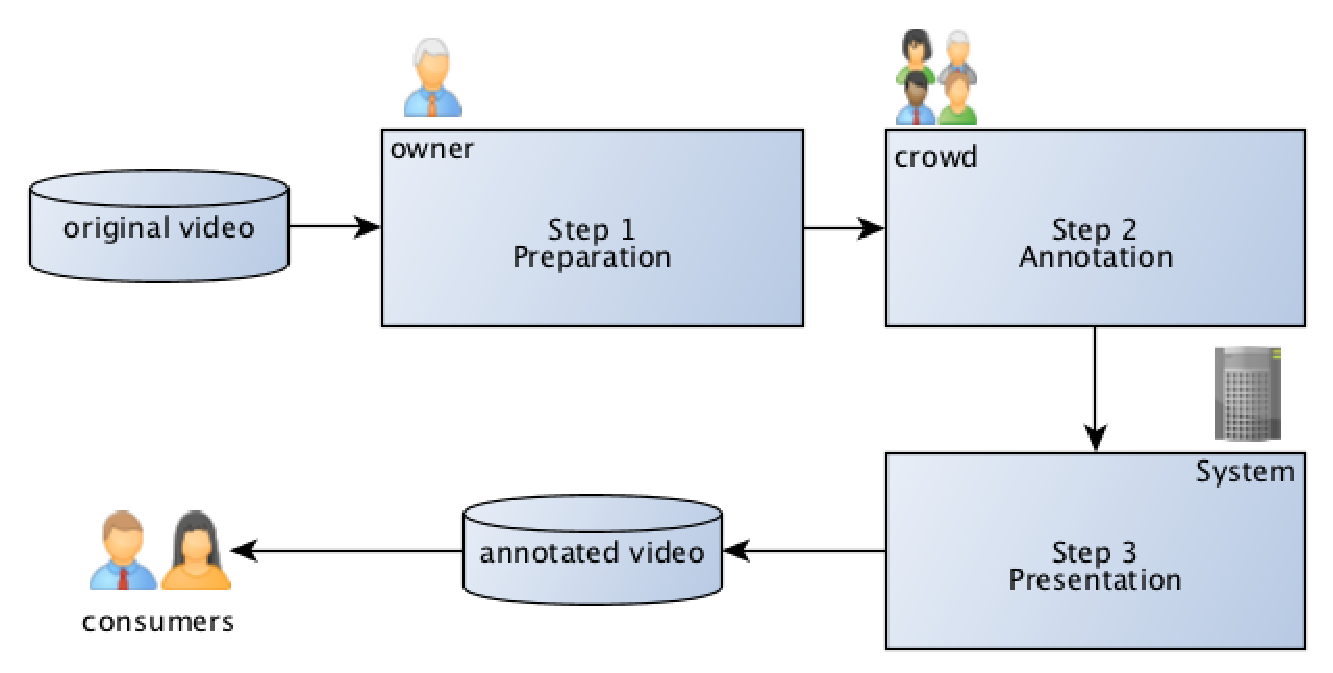
\includegraphics[scale=0.4] {figure/process}}
	\caption{Process workflow}
	\label{process}
\end{figure}

\textbf{Preparation:} all activities involved in this step are performed by the owner, who started the video annotation process. At this step is determined what must be annotated, also how they should be annotated. In this way the owner must determine:
\begin{enumerate}
\item What kinds of point of interest should be annotated.\\Ex: events, objects, subjects, issues.
\item What annotation type will be used for each of these kinds.\\Ex: free write, item select, button click, image upload.
\item What data type will be collected for each annotation type.\\Ex: plain text, location, image, video.
\end{enumerate}

To illustrate this point, the example of the football(soccer) match annotation will be recalled. In a football(soccer) match video the kinds of point of interest correspond to events such as goals, cards and faults. For each point of interest observed it should be collected its kind, and the instant when this event happened. The annotation type to be used on the annotation tool can be a set of icons related to each event. Finally, the data type collected in this case may be plain text that contains the kind of event identified and the instant it happened \cite{santos2007estrategia}.

Also it is important to provide explanations or guidelines that can instruct the workers about how execute the microtasks. An additional activity on the Preparation step is determine what section of the video should be send by each worker, this division can be made by duration (ex: send a 5 seconds segment to each worker), or using contextual criteria such as to send to each user a segment that contains a single dialog. The activities sequence for this step can be observed on Figure~\ref{preparation}.

\begin{figure}[h]
	\centerline{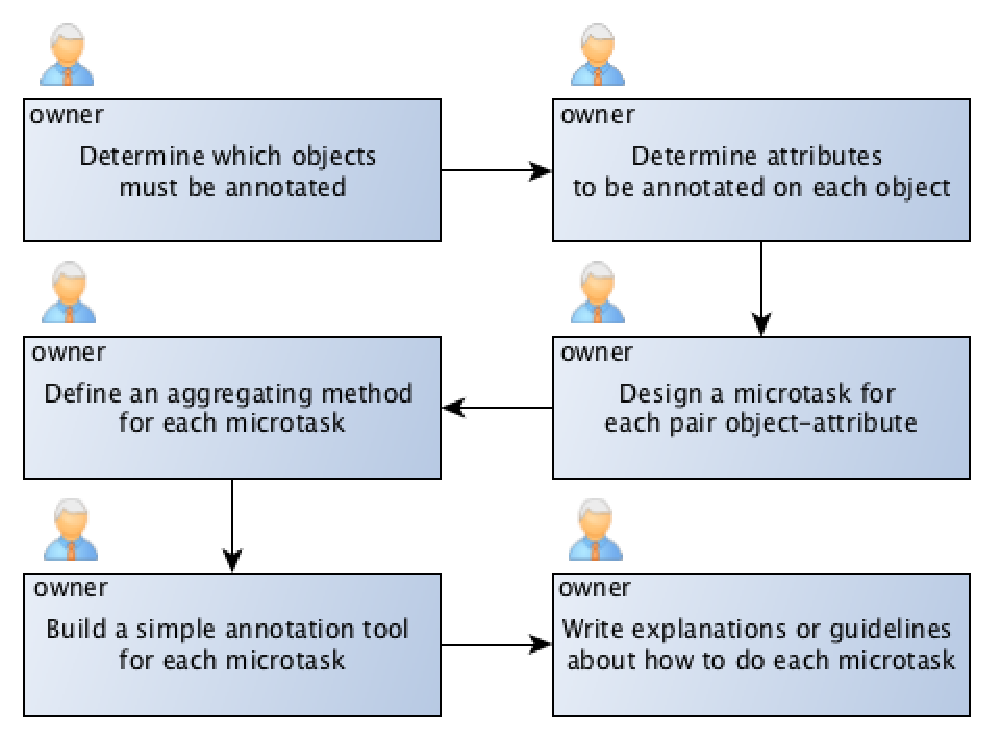
\includegraphics[scale=0.4] {figure/preparation}}
	\caption{Preparation step}
	\label{preparation}
\end{figure}


\textbf{Annotation:} an essential aspect for this step is to determine the microtasks' workflow, so the output from a task is taken as input by the next one, generating a final outcome at the end of the last microtask. This cascade workflow is illustrated in Figure~\ref{cascading}. It is important to notice that each task cell in composed by two activities, the microtask in self and the aggregation method, that generates the output from the obtained contributions. In this way, the output from the last task cell is the final outcome provided by the system.

\begin{figure}[h]
	\centerline{\includegraphics[scale=0.25] {figure/cascading}}
	\caption{Annotation step for N microtasks}
	\label{cascading}
\end{figure}

\textbf{Presentation:} at this step is generated an annotated video including the original video and the final outcome from the previous step. Other activities that can be proceeded at this step is to generate, or to render, media items selected from the crowd annotations, as well as aggregate these items over the videos to compose a multimedia presentation.

\begin{figure}[h]
	\centerline{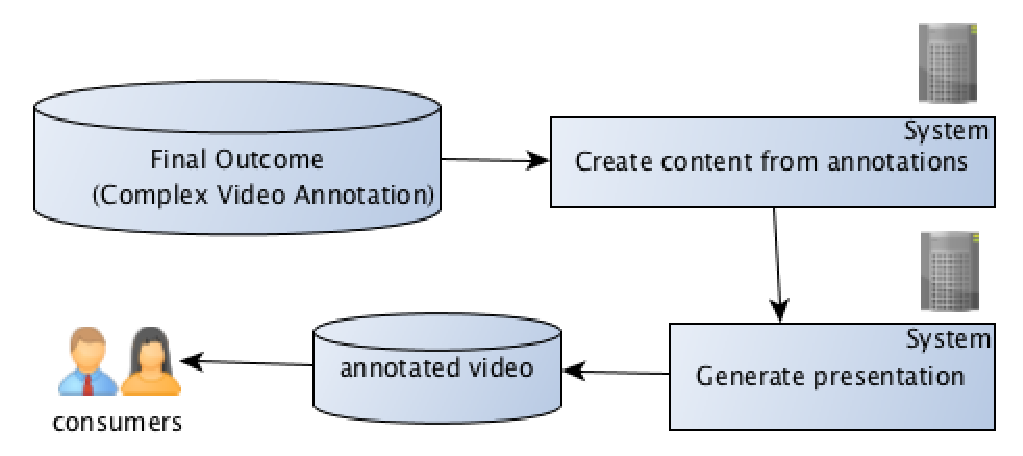
\includegraphics[scale=0.5] {figure/presentation}}
	\caption{Presentation step}
	\label{presentation}
\end{figure}










\section{Experiment}
	\begin{figure*}[ht]
	\centerline{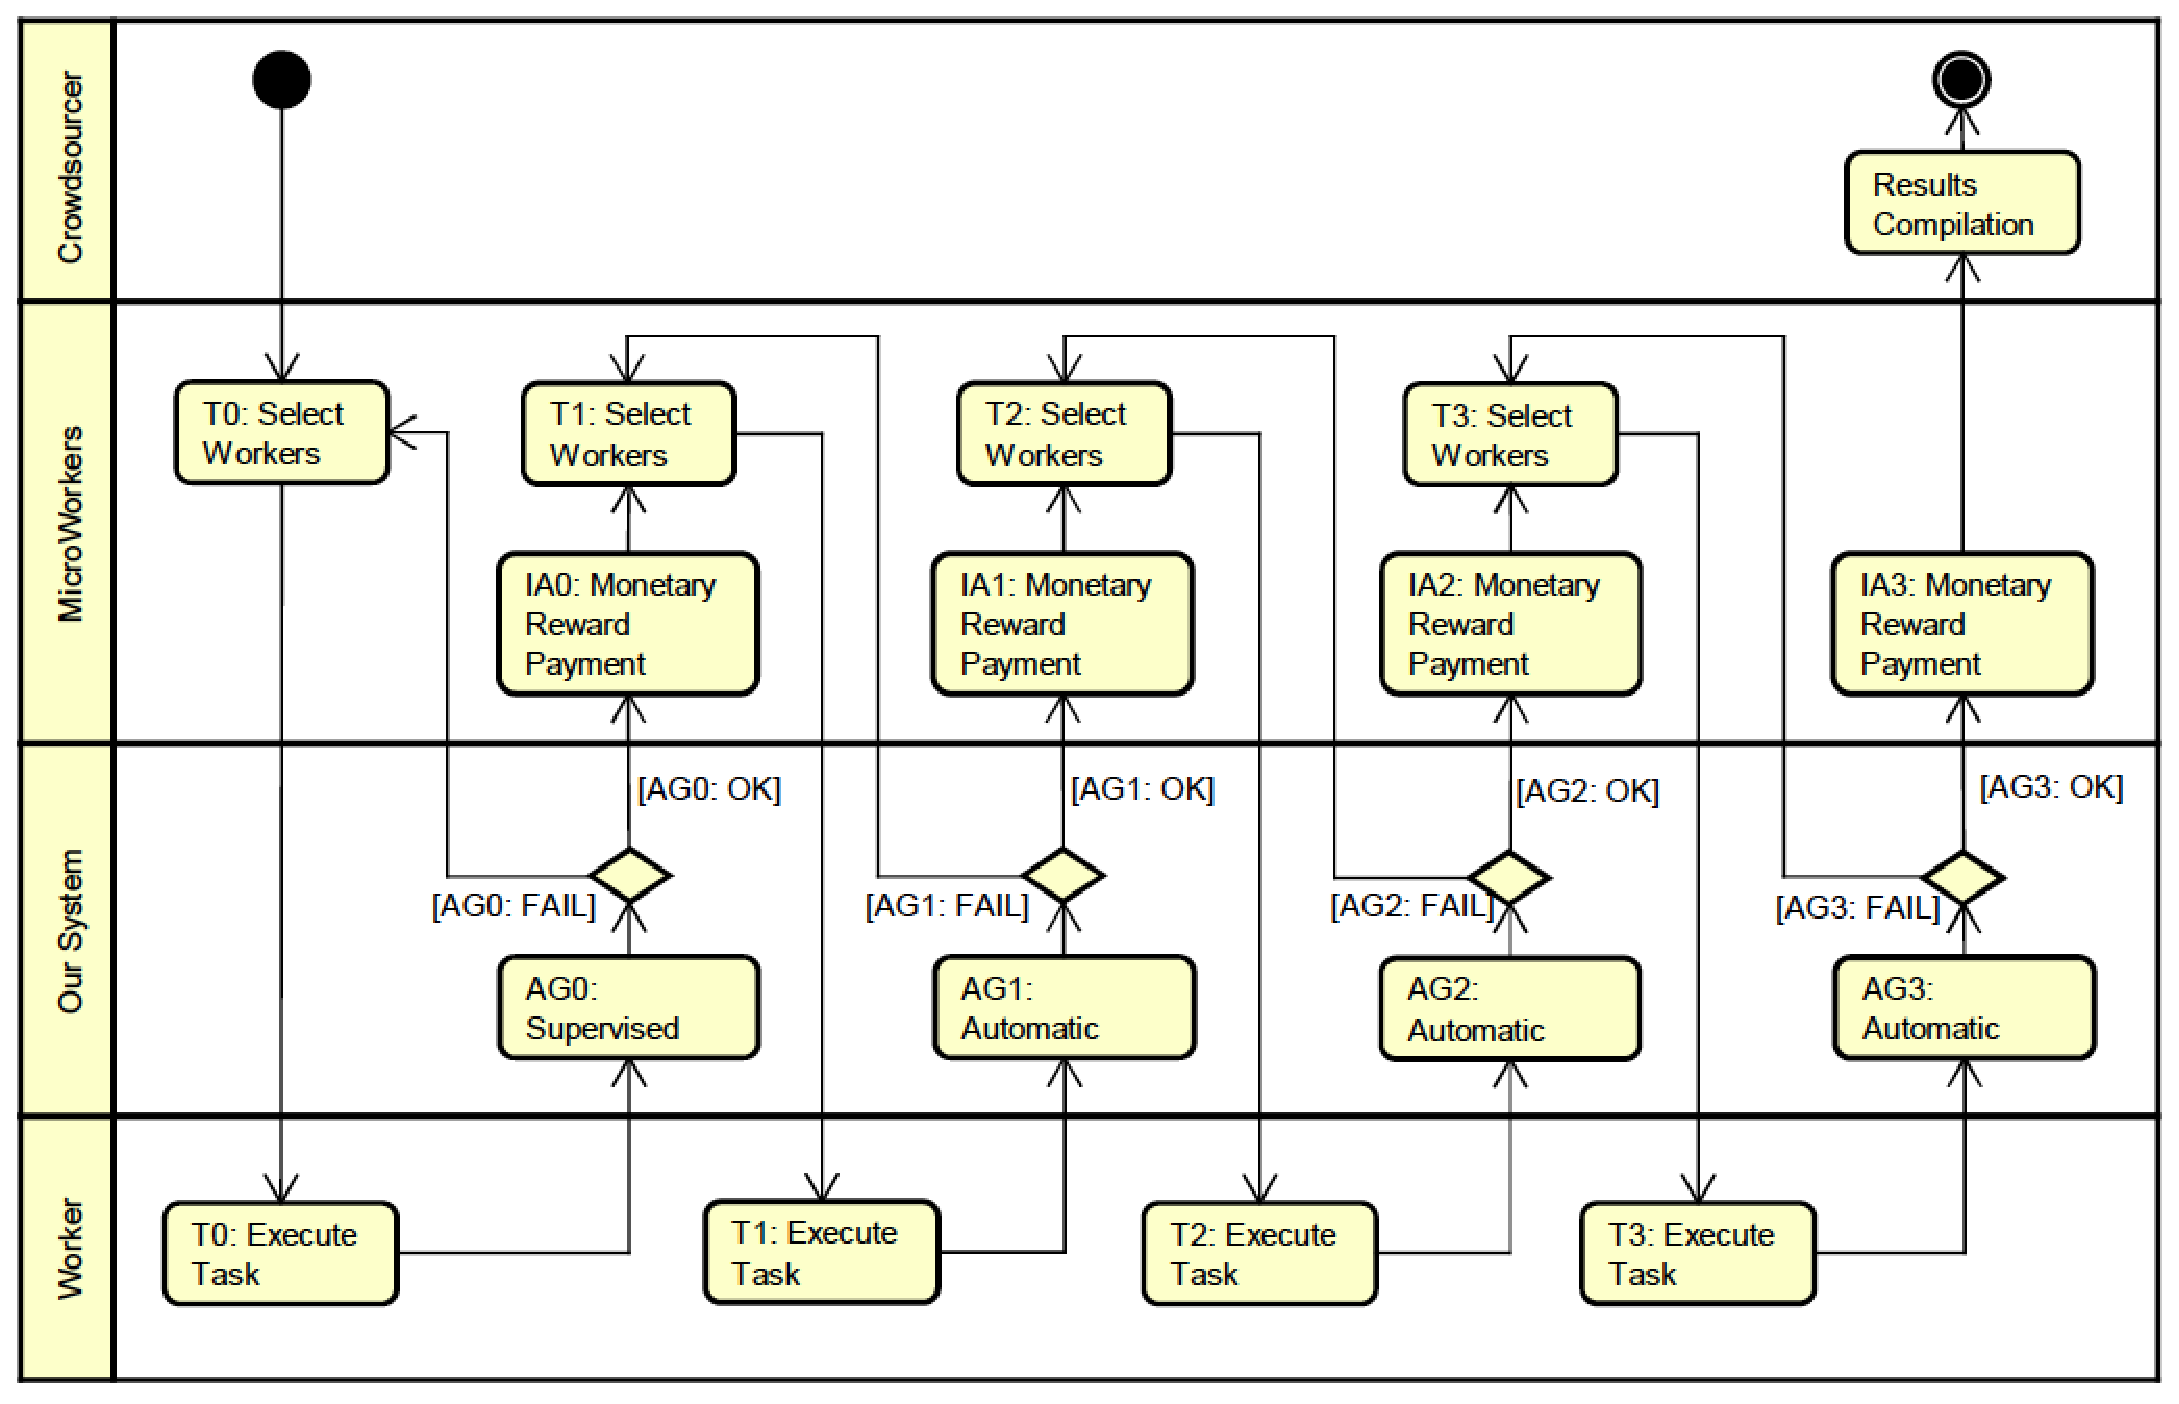
\includegraphics[scale=0.35] {figure/case}}
	\caption{Video Enrichment Workflow. T (Task); AG (Aggregation); IA (Incentive Application).}
	\label{workflow}
\end{figure*}

This experiment used the presented method to enrich videos by adding semantic information about personalities, theories, and technologies in an explanatory video about the history of computation. 

%The rich video generated is a self-contained multimedia document, so the user doesn't need to access supplementary content from other sources.

%Each supplemental content can be accessed through trigger items that are images and labels that appear in scenes where the point of interest is mentioned. When the trigger items are clicked, the video pauses the extra content is displayed so they can be viewed, and when closed, video playback resumes normally.

The crowdsourcing process used in the experiment followed a workflow of four annotation microtasks. Each of these simple tasks was modeled that could be performed by a worker through a simple annotation tool. The video features an actress narrating a text about the history of computing.
%The video produced for the experiment shows an actress narrating an English text.
%The video was produced in the English language and features an actress narrating a text about the history of computing.

%Preparation and Annotation processes, including workflow construction, microtasks definitions, annotation tools, the aggregation methods, as well the results obtained in each microtask will be described below.

\subsection{Our Crowd}
To reach a heterogeneous crowd we used the Microworkers platform to recruit and pay workers, and the whole process was supported by our framework.

Microworkers proposes different models for a crowdsourcing process. Initially, you can choose between starting a basic campaign or using contracted groups. In a basic campaign, all registered workers in the system can see the task on the job wall and accept to run it. A campaign that uses hired groups allows you to select the crowd by choosing groups of workers with a certain profile. In addition, it is possible to create lists with good workers who have made good contributions to recruit them for other tasks. 
%Some of hired groups available in Microworks are listed in Figure~\ref{groups}.
%\begin{figure}[h!]
 %\centerline{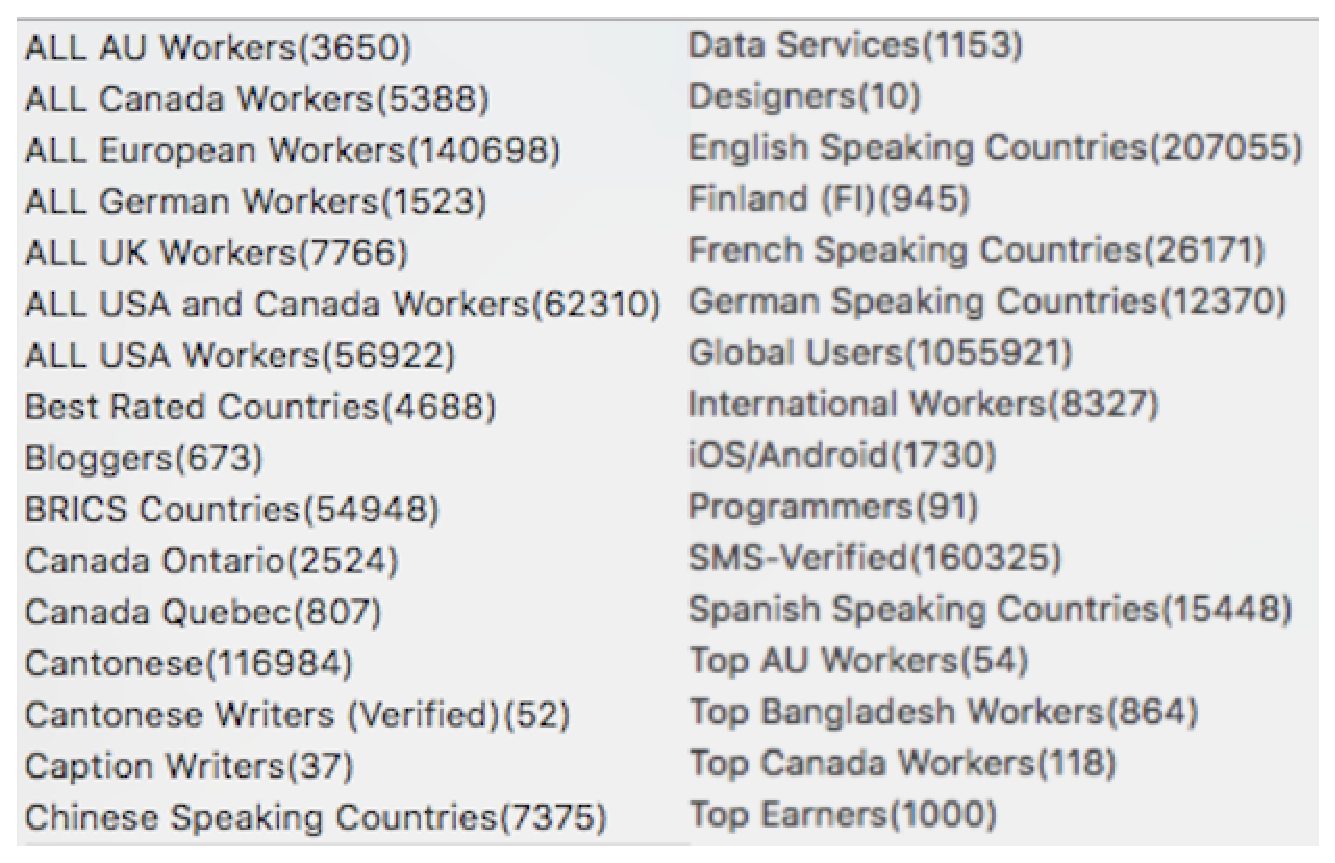
\includegraphics[scale=0.25] {figure/groups}}
%	\caption{Microworkers Hired Groups}
%	\label{groups}
%\end{figure}

The purpose of this paper is to use unskilled workers, although it was necessary for them to know enough of the English language to understand the video used in the experiment. For that reason, the tasks were launched as campaigns that used contracted groups, to increase the chance of the workers who contributed in a task also participate in others, was chosen a group of moderate size and with workers relatively assiduous so that the contributions were made quickly. The group chosen was Data Services, with 1153 potential workers to accept the jobs.

Some groups are made up of workers who only accept tasks that offer slightly larger payments, but considering the group chosen, it was feasible to offer a payment of 0,02 USD per task. Also, each task was active for 24 hours to reach all time zones in the same way.

\subsection{Preparation}

The preparation step began with the identification of the micro-tasks needed to achieve the expected result. Since the goal was to generate enriched videos through supplementary content at points of interest, it was determined that they were needed. Thus, it was determined that four microtasks would be performed:

\begin{itemize}
\item Identify the points of interest in the video; 
\item Gather content suggestions for each point of interest; 
\item Select the best extra content to each point of interest;
%Determine the most accepted supplementary content for each point of interest; 
\item Position the trigger items at the best spot over the video. 
\end{itemize}

Related to the items distributed to be annotated in each task, a circular list policy was adopted. In this way, there was a greater chance of each task, each item being annotated received the same number of contributions.

It was also necessary to determine how the video should be segmented to generate the input of the first task. The strategy chosen was to target the video based on the automatic captions generated by Youtube\footnote{https://youtube.com}. In this way, it was possible to generate short segments, but they tend to contain complete sentences. This method divided the video into 13 segments.

For budget and time issues, it was determined that the minimum amount of contributions each item could receive was five, so Task 0 should receive at least 75 contributions. The number five was chosen because it is odd, which avoids drawings, and because it is an amount that already allows seeing a tendency of convergence of opinion in a heterogeneous multitude.



\subsection{Annotation}
In this section will be described the 4 annotation tasks, as well the annotation tools, aggregation methods and results for each of them. Because there is a dependency order between these tasks, it's not possible run them in parallel. In this way, an execution workflow in which the output of one task is used for the next one, as can be seen in Figure \ref{workflow}.
%\begin{figure*}[h]
%	\centerline{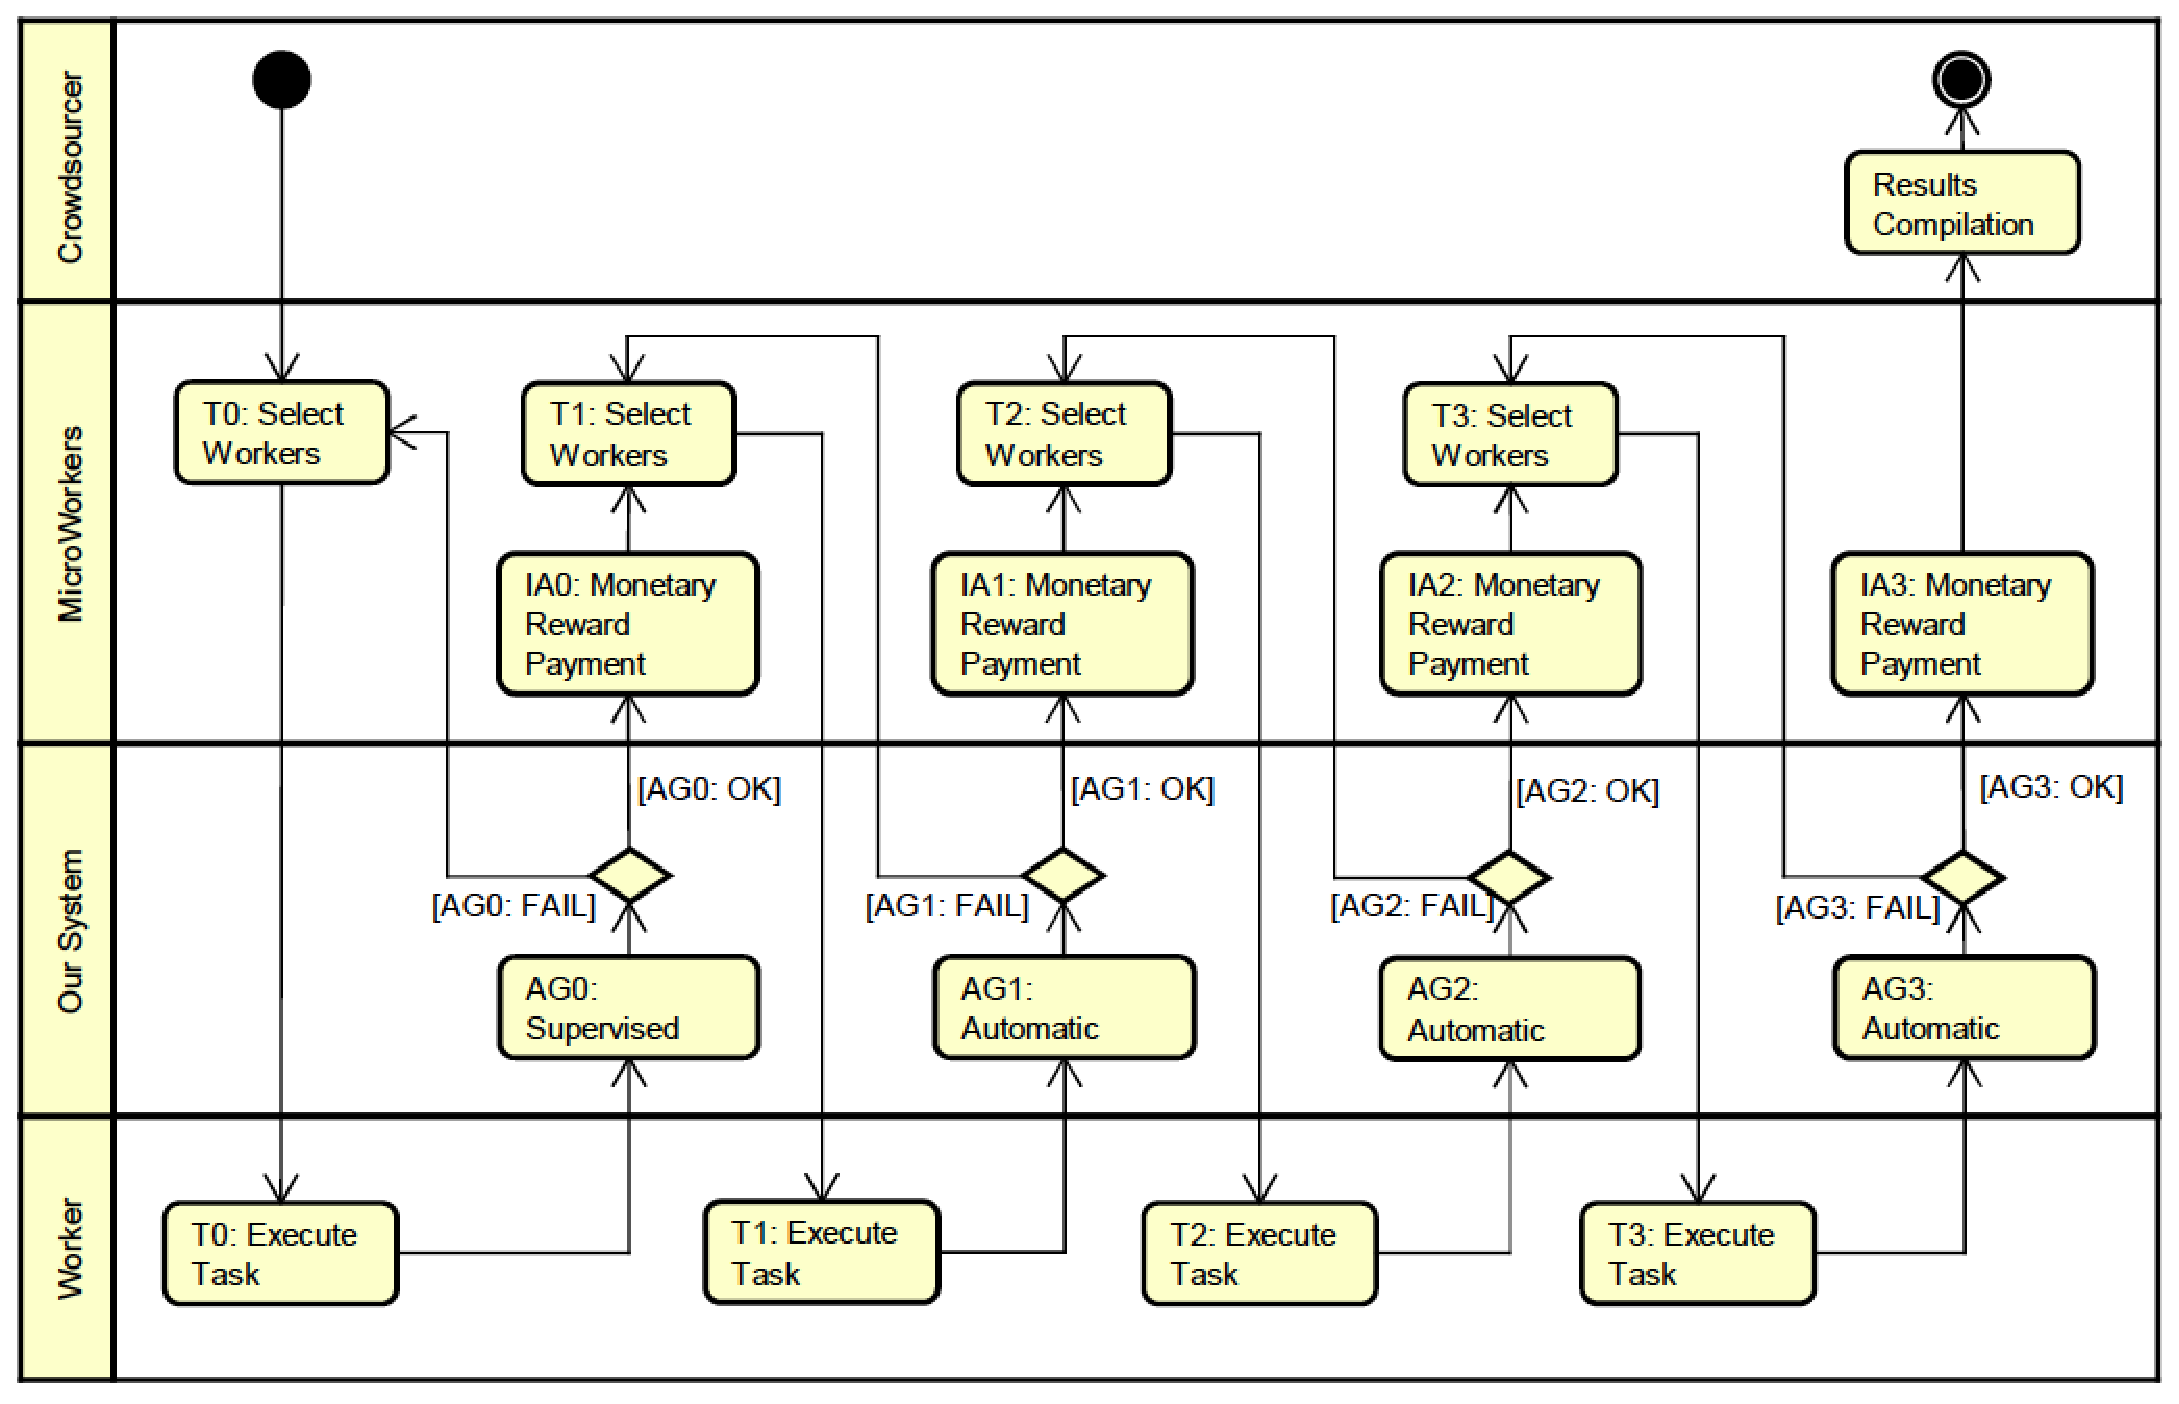
\includegraphics[scale=0.235] {figure/case}}
%	\caption{Video Enrichment Workflow}
%	\label{workflow}
%\end{figure*}

%Each of the four tasks applied to the workers will be described below, as well presented the annotation tool used for them.

\subsubsection{Task 0}
%\textbf{Identify Points of Interest:} The first annotation microtask is supported by the tool represented in Figure~\ref{task_1}, collecting identification for points of interest. In this task, the contributor receives a segment of video that should be watched, and if was found any point of interest, it should be marked and briefly described. These points of interest can be gestures, words, expressions, facts, concept, characters, events or anything that can be related to extra content.


\begin{itemize}
\item \textbf{Title:} Identify Points of Interest.

\item \textbf{Description:} A video segment is displayed to the worker and he must identify the moment at which a point of interest appears or is mentioned. This point of interest can be a person, a technology or a theory.

\item \textbf{Objective:} Identify points of interest in a video segment.


\item \textbf{Input:} A dataset with 13 video segments of 4.5 to 7 sec.


\item \textbf{Output:} A set of points of interest and the instant when they happen. In addition to serving as input to Task 1, this result also generated a summary based on points of interest.


\item \textbf{Instructions:} \begin{enumerate}
	\item Identify in the video something that you found interesting.
	\item Pause the video the moment it appears.
	\item Select its type: Person, Technology or Theory.
	\item Write what you have identified. 
\end{enumerate}

\item \textbf{Annotation Tool:} The tool is represented in Figure~\ref{task_0}.
\begin{figure}[h!]
	\centerline{\includegraphics[scale=0.17] {figure/task_0}}
	\caption{Annotation Tool for Task 0}
	\label{task_0}
\end{figure}

\item \textbf{Aggregation:} For this task, a supervised aggregation method was chosen in which the human interaction occurs at the end of the process. The contributions are filtered discarding the useless contributions (empty, nonsense, bad works), and the valid contributions are candidates to Points of Interest. The candidates are grouped in two-seconds interval ranges. In each group, a similarity analysis is done and the most frequent occurrence is selected. Finally, the human supervisor edits the selected label so that the text is visually pleasing. The aggregation method extracted 11 Points of Interest from the 75 contributions.

\end{itemize}



\subsubsection{Task 1}

%\textbf{Provide extra content suggestions:} The second task took as input the aggregated result from the task 1 that is a list of points of interest identified by the workers. This microtask is supported by the annotation tool represented in Figure~\ref{task_2}. This tool presents to the worker a point of interest and the video segment positioned at the moment it occurs. This way, is possible to use the video for reference and contextualization.



%Through this tool, the worker can contribute by writing a text related to the point of interest, sending an image or sending a link to a YouTube video or a Wikipedia page.


%When the collection of contributions for this task is done, the Aggregator groups the content of the sender by a point of interest, and then joins the similar suggestions. In this way, a list of points of interest with a set of content suggestions for each is added to the next task, without repeated suggestions.

\begin{itemize}

\item \textbf{Title:} Provide Suggestions for Extra Content.

\item \textbf{Description:} In this task, the worker receives a point of interest and the video synchronized at the moment it occurs. The worker should suggest extra content to complement the video, which may be a short text, an image or a link to a YouTube video or a Wikipedia page.

\item \textbf{Objective:} Obtain from the crowd extra content to each point of interest.


\item \textbf{Input:} The set of points of interest collected in Task 0.


\item \textbf{Output:} A set of extra content associated with each point of interest. Each extra content may be an explanatory text, an image, even a link to a Wikipedia page or a Youtube video. Besides feed the Task 2,this output is also used to generate a content-based index to the video.


\item \textbf{Instructions:} \begin{enumerate}
	\item Select the type of content to send.
	\item You can upload an image, write a short text.
	\item You also can paste a link to Youtube or Wikipedia.
\end{enumerate}

\item \textbf{Annotation Tool:} The tool is represented in Figure~\ref{task_1}.
\begin{figure}[h!]
	\centerline{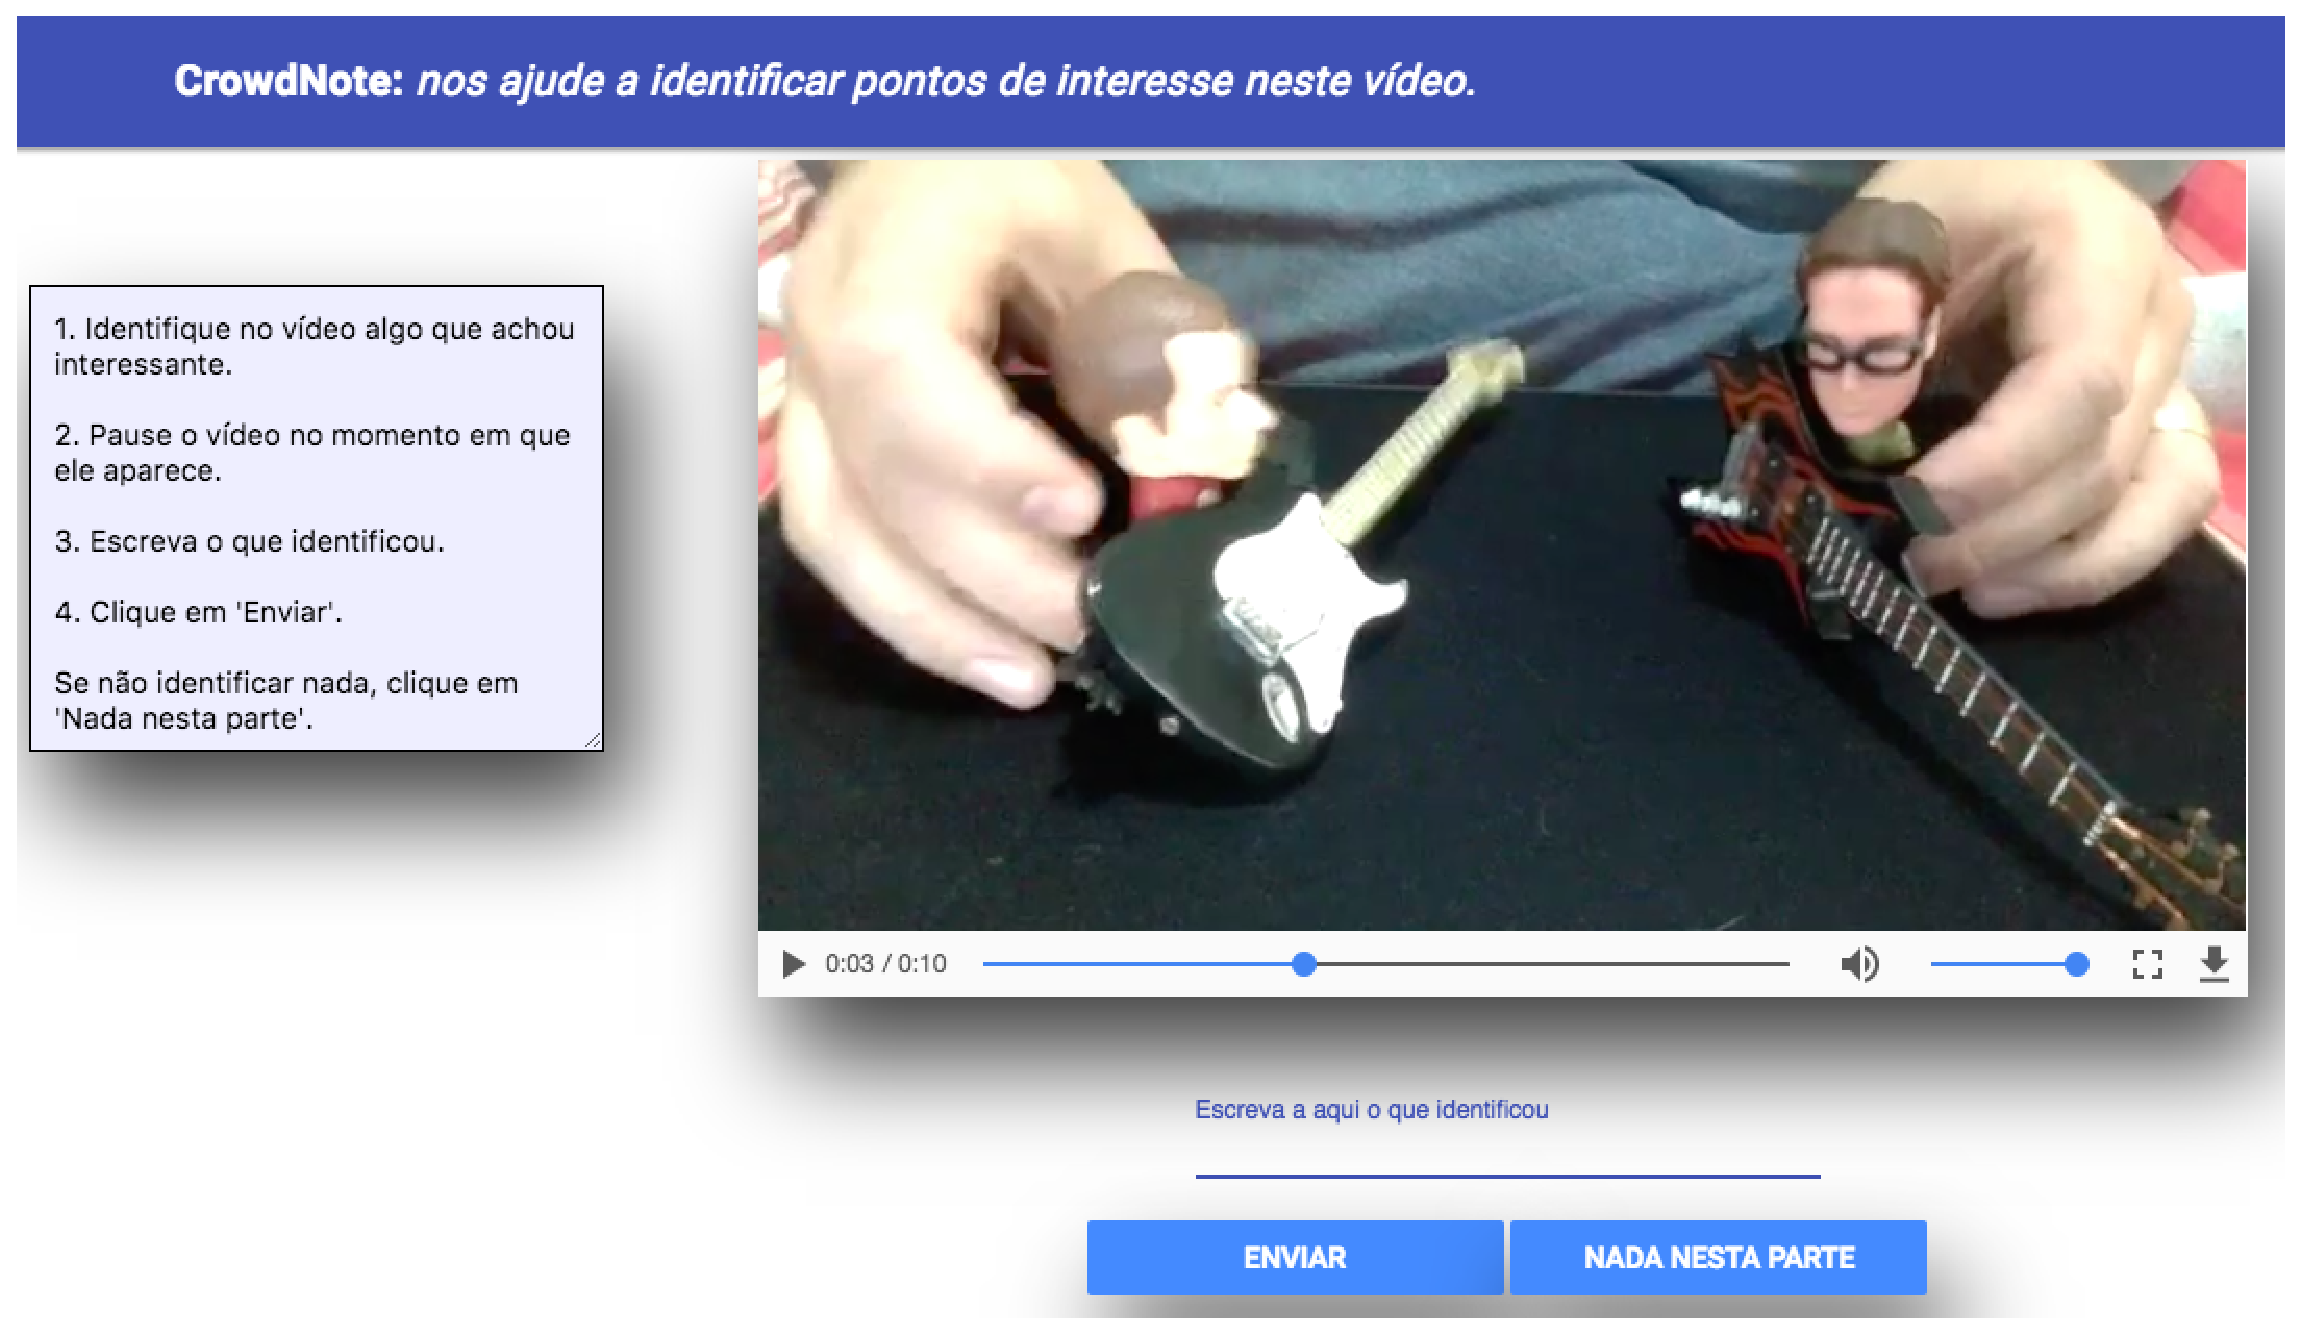
\includegraphics[scale=0.165] {figure/task_1}}
	\caption{Annotation Tool for Task 1}
	\label{task_1}
\end{figure}

\item \textbf{Aggregation:} For this task was chosen an automatic aggregation method. The filtering step discarded the corrupted files and broken links. The suggested contents were grouped by point of interest, and the duplicated items were merged. The aggregation method extracted 34 different suggestions of extra content from the 55 contributions received. All 11 points of interest received at least two content suggestions, some of which received four or five. 
%The ideal case would be to obtain a more even distribution, although the result obtained was enough to continue the process.

\end{itemize}



\subsubsection{Task 2}



\begin{itemize}

\item \textbf{Title:} Ranking Suggestions.

\item \textbf{Description:} The worker receives a point of interest and the video positioned at the moment it occurs. It also gets the list of suggested extra content to complement this point of interest. The job is to choose the extra content that best complements the content related to the point of interest.

\item \textbf{Objective:} Determine the best extra content to each point of interest, according to the crowd.


\item \textbf{Input:} A set of points of interest, with the suggested contents associated with each one.


\item \textbf{Output:} An updated set of points of interest with the extra contented associated with each one. This output also can be used to generate a ranked list of alternative extra contents to supplement the points of interest.


\item \textbf{Instructions:} \begin{enumerate}
	\item Use the buttons bar to navigate through the contents.
	\item You can use the zoom button to visualize each content.
	\item Vote for the content you liked best.
\end{enumerate}


\item \textbf{Annotation Tool:} The tool is represented in Figure~\ref{task_2}. This tool has a drag-and-drop feature that lets you drag the item through the video until you find the appropriate position.
\begin{figure}[h!]
	\centerline{\includegraphics[scale=0.165] {figure/task_2}}
	\caption{Annotation Tool for Task 2}
	\label{task_2}
\end{figure}

\item \textbf{Aggregation:} This simple automatic aggregation method determines the most popular extra content suggested to each point of interest. As the contents were associated with 11 points of interest, were collected 55 contributions. In the filtering step the suggestions without votes was discarded. Finally, was generated an output with all 11 points of interest and the extra content associated with each one. 

\end{itemize}



\subsubsection{Task 3}

\begin{itemize}

\item \textbf{Title:} Determine the Position of the Trigger Items.

\item \textbf{Description:} This task consists of placing a trigger item in a video scene. This trigger item is represented as a rectangle containing a text or an image and should be positioned so as to minimize occlusions of important scene objects.

\item \textbf{Objective:} Determine the best position to display each trigger item over the video.


\item \textbf{Input:} A set of points of interest with the extra content associated with each one of them.

\item \textbf{Output:} Aset of points of interest with the extra content associated with each one, including now the position where each item should be displayed over the video. These positions are represented as coordinates (X,Y). The output of this task is the outcome of the video enrichment process, and can be executed in the Player. In addition, the metadata can be used to generate alternative outputs such as NCL to reproduce them in digital TV environments.


\item \textbf{Instructions:} \begin{enumerate}
	\item Drag the item by the video until finding the best position.
	\item When you have decided on the best position, click send.
\end{enumerate}


\item \textbf{Annotation Tool:} The tool is represented in Figure~\ref{task_3}.
\begin{figure}[h!]
	\centerline{\includegraphics[scale=0.17] {figure/task_3}}
	\caption{Annotation Tool for Task 3}
	\label{task_3}
\end{figure}

\item \textbf{Aggregation:} The automatic aggregation method applied at the final of this task determines the position at each item should be displayed over the video. The contributions for each item were grouped and the very discrepant positions of the others were discarded. Then, for each item, the average geographic position was calculated based on the X and Y coordinates predicted in the contributions. Was collected 55 contributions, of which 38 were after filtering. Of these 38 contributions were extracted the positions of the 11 items related to the points of intersection.

\end{itemize}


\subsection{Presentation}

The presentation system, shown in Figure~\ref{player}, receives the video, extra content, and necessary metadata from the Player Provider. This system is capable of reproducing the original video synchronized with the extra content, that is displayed every time a point of interest happens in the video. Is important to remind that all extra content displayed with the video was provided, selected and positioned by the crowd.



\begin{figure}[h!]
	\centerline{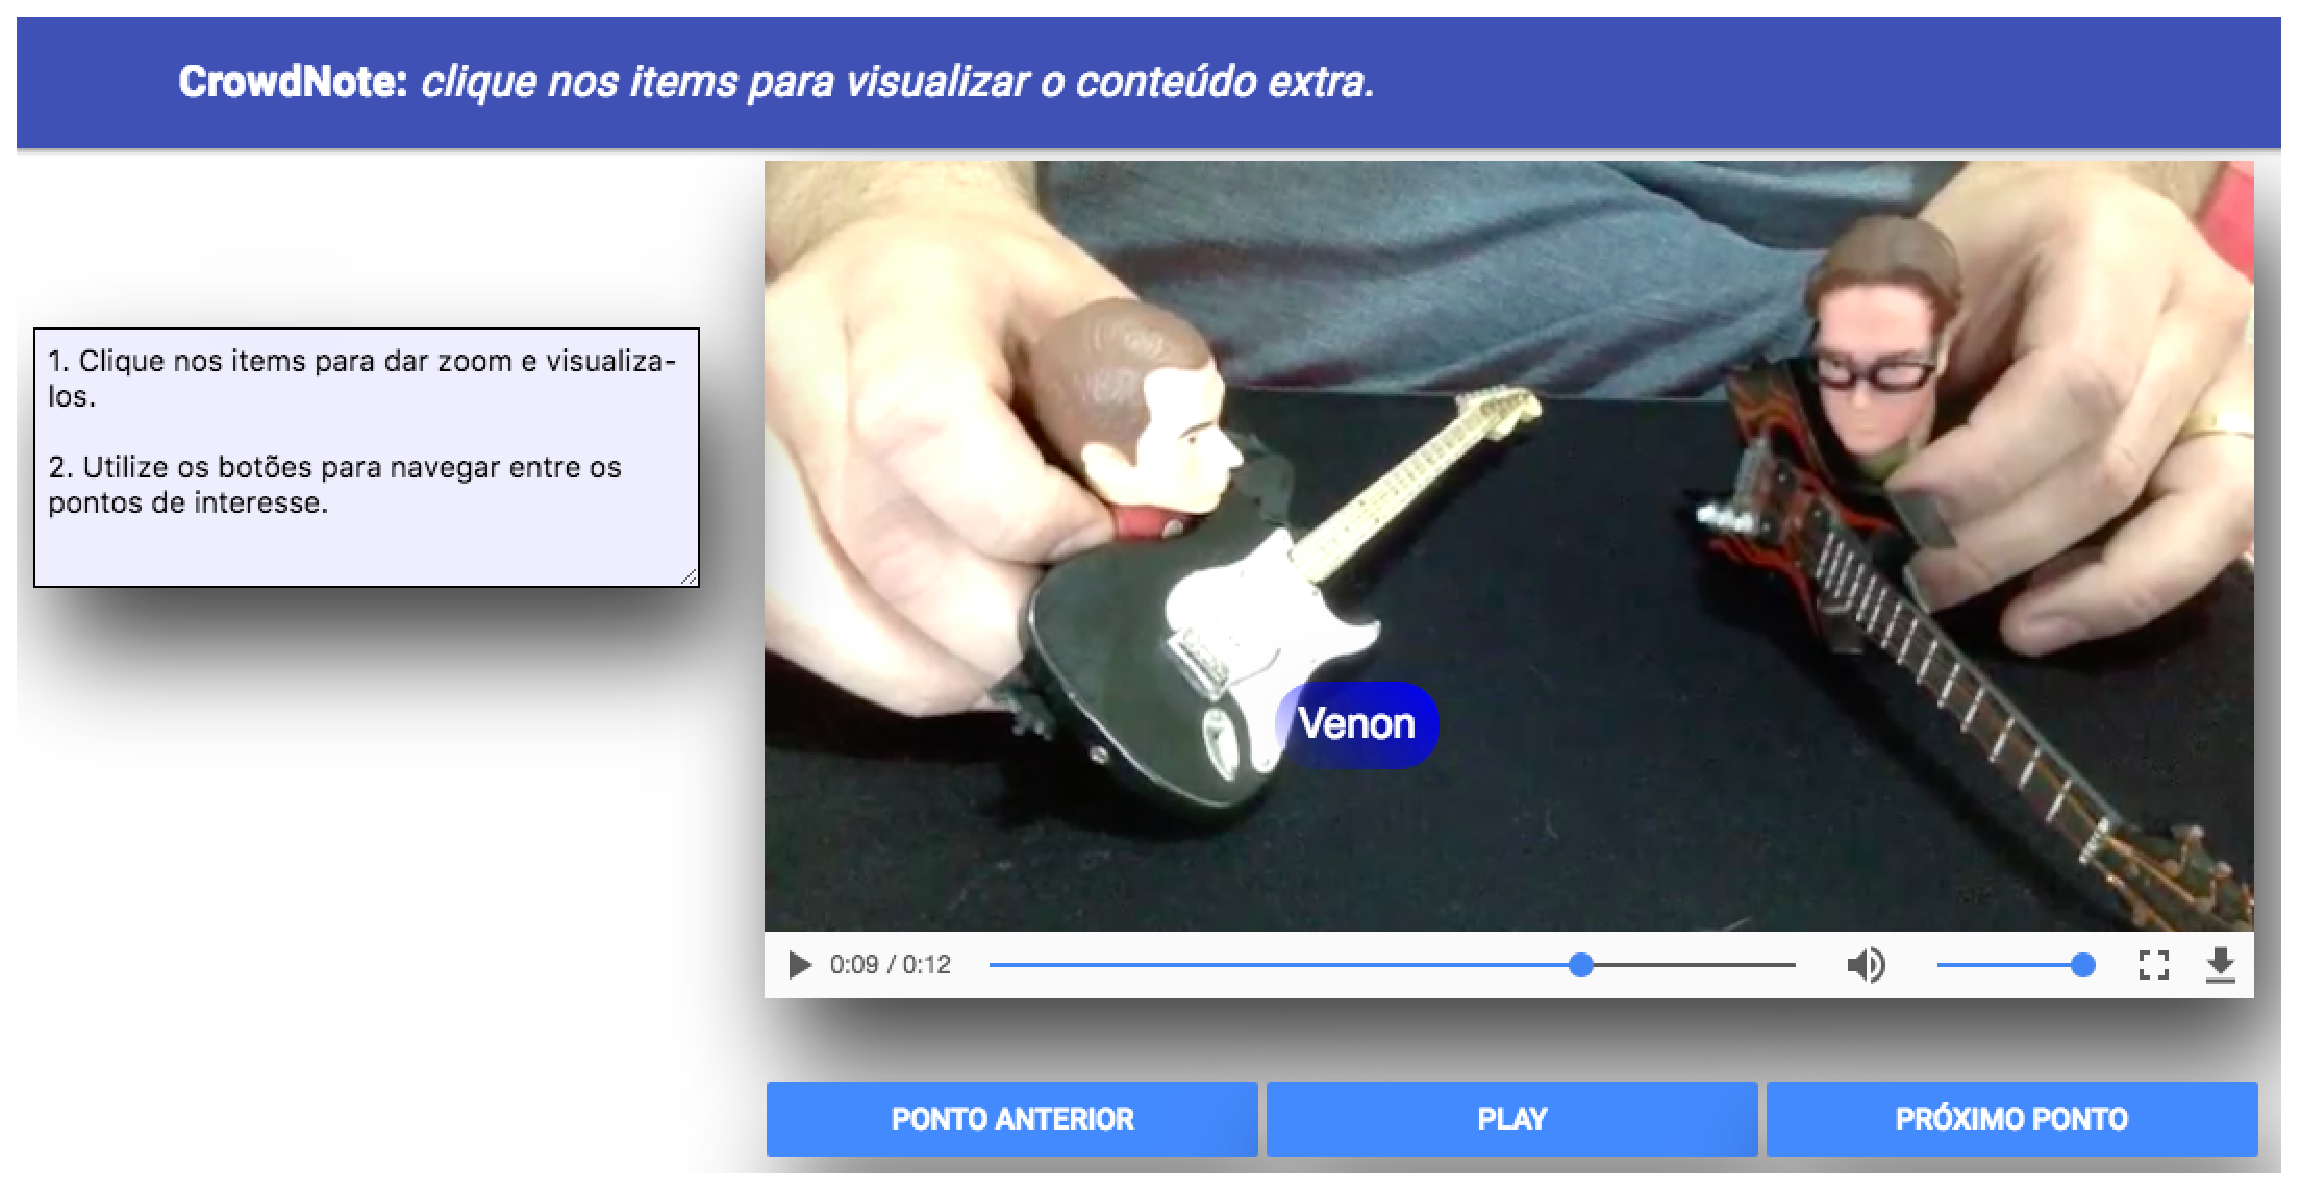
\includegraphics[scale=0.17] {figure/player}}
	\caption{Displaying an extra content item over the video}
	\label{player}
\end{figure}

This tool has a control bar with 3 buttons: Previous, Next and Zoom. These buttons are used to control two useful features, the content zoom and the navigation by point of interest.

The navigation by point of interest uses the list of points as a content index, allowing the user to navigate between points of interest by clicking the Previous and Next buttons. The Player automatically syncs the video at the time the current point of interest occurs.

When the user clicks the trigger item or the Zoom button, the extra content associated with the current point of interest is displayed on an upper layer as the video is paused. When you close the extra content, the video resumes its execution from where it was. The zoom view can be seen in Figure~\ref{player_zoom}.

\begin{figure}[h!]
	\centerline{\includegraphics[scale=0.17] {figure/player_zoom}}
	\caption{Player Zoom}
	\label{player_zoom}
\end{figure}



 \subsection{Runtime Observations}
 
During some tasks, we observed some interesting facts about the behavior of workers. Keeping in mind that the motivation of the workers in the experiment was the payment and that the amount paid for each job was small, the workers tended to do the bare minimum. This aspect proved to be correct that the decision was made to use microtasks that needed only a simple interaction to be completed.
 
The reflection of this led to some decisions during the experiment, as in Task 1. In this task, the worker were asked to suggest extra content to supplement the points of interest and for this, he could write a short text, paste a link to Wikipedia or Youtube, or upload an image. Most workers provided links and only two uploaded images. We thought that the reason was because sending an image was more laborious than pasting a link into the text box, as it was necessary to download the image and upload it.

However, this occurrence was used positively, because few image was obtained in the contributions, so, decided to add an automatic mechanisms to retrieve them automatically during aggregation. In cases where the selected point of interest was a Wikipedia link mechanism, it retrieved the main page image and, in cases where it was linked to YouTube, the thumbnail was retrieved from the video.

Although this operation is simple, it shows that it is possible to improve the aggregation methods by associating more automatic processing with human contributions. In this way, aggregation methods may be possible integration points with other systems, even with secondary human tasks to create a formal model of supervised aggregation activity.

\subsection{Result Evaluation}
The rich video generated is a self-contained multimedia document, so the user doesn't need to access supplementary content from other sources.

Each supplemental content can be accessed through trigger items that are images and labels that appear in scenes where the point of interest is mentioned. When the trigger items are clicked, the video pauses the extra content is displayed so they can be viewed, and when closed, video playback resumes normally.

This outcome was evaluated according three criteria: points of interest identified, suitability of the associated content, and occlusion of scene objects.

According to the author of the video used in the experiment, there were 21 different points of interest, which after aggregation would result in 14, because at each interval of two seconds, only the most relevant point of interest would be selected. The crowd managed to identify 19 points of interest, which after the aggregates generated 11 relevant points. However, the crowd highlighted the term "Formalism" that  was not predicted by the author, who after checking it reported that it was valid in the video's context.

The extra content selected for each point of interest was also verified by the author. Of these, only one content did not meet the author's expectations. The content selected for "Logical relations and properties" corresponded to what the author wanted to convey. However, he realized that there was a flaw in the video script and the correct text would be "logical relational and its properties". This way this error can not be attributed to the crowd.

In relation to the occlusion of the objects of the scene, the criterion to calculate items that were positioned in the actress who narrated the text. Of the 11 items, only 2 slightly obscured the outline of the actress, as shown in Figure~\ref{oclusion}, but no item occluded her image significantly.

\begin{figure}[h!]
	\centerline{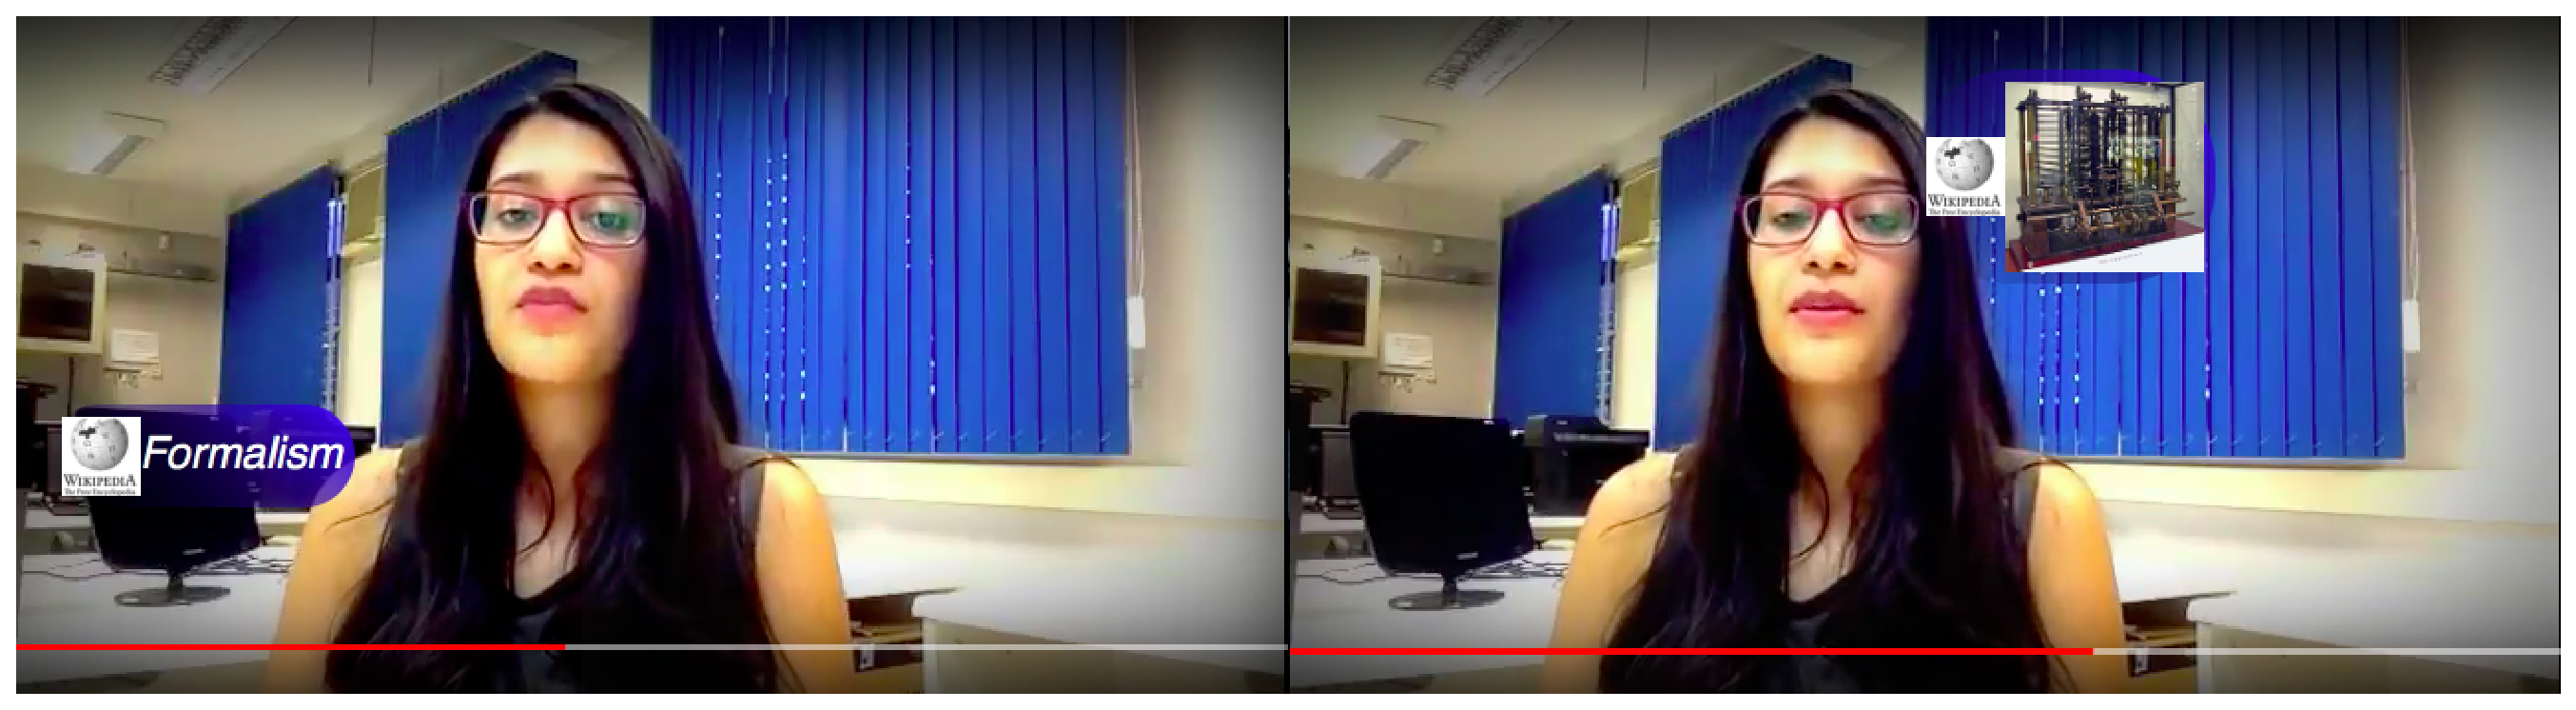
\includegraphics[scale=0.19] {figure/occlusion}}
	\caption{Occlusion Issues}
	\label{oclusion}
\end{figure}

In general, the result generated by the crowd was well adapted to convey the content intended by the author, having enriched virtually all the points that he had predicted. Finally, the result of our experiment demonstrate that the crowd is capable of generating dependable additional content to improve videos. The result of our case study can be seen in the player of our framework\footnote{http://159.203.171.150:83}.





















\section{Conclusion}
	
This paper presented a method for achieving a complex media annotation by running a process workflow composed of simple annotation microtasks in a cascading arrangement. 

%Some relevant improvements were made to both the method and the framework used to support its activities.

%The contribution of this manuscript is twofold. Firstly, we have improved the cascading process proposed in [REMOVED FOR BLIND REVIEW]. Secondly, YYY


Although more studies are needed, the experiment showed in the first analysis that the cascading method based on microtasks can produce an annotated content that is coherent and comparable to the one produced by an experienced annotator. The worker's contributions were obtained from a commercial crowdsourcing environment, but with a differentiated approach in which only the resources related to the workers and none of the platform resources were used. This approach ensured that both the data set used and the data collected in the contributions were stored only in our database, not the crowdsourcing platform.


It was also observed that the concept of supervised aggregation introduced in this paper obtained positive results. This aggregation approach has proven to be interesting for improving the results of annotation tasks that receive open answers that need to be adjusted manually. A direct conclusion is that this approach can also be used to insert a human verification step at the end of certain aggregation activities.

%The diagrams introduced considerably facilitated the creation of the workflow from the production process to the case study. In addition, a specification of the dataflow in the interfaces between the components, facilitating the planning of the distribution of the works and the information that is necessary.

%The basic annotation tools distributed with the framework can be easily adapted to work with the commercial crowdsourcing platform as well as to meet the requirements of the tasks required for the experiment.

%As can be seen in Figure \ref{workers}, the workers who contributed to the experiment are scattered all over the world. This ensured a heterogeneous crowd, which contributed to the operation of aggregation methods based on the wisdom theory of the crowds.
%\begin{figure}[h]
%	\centerline{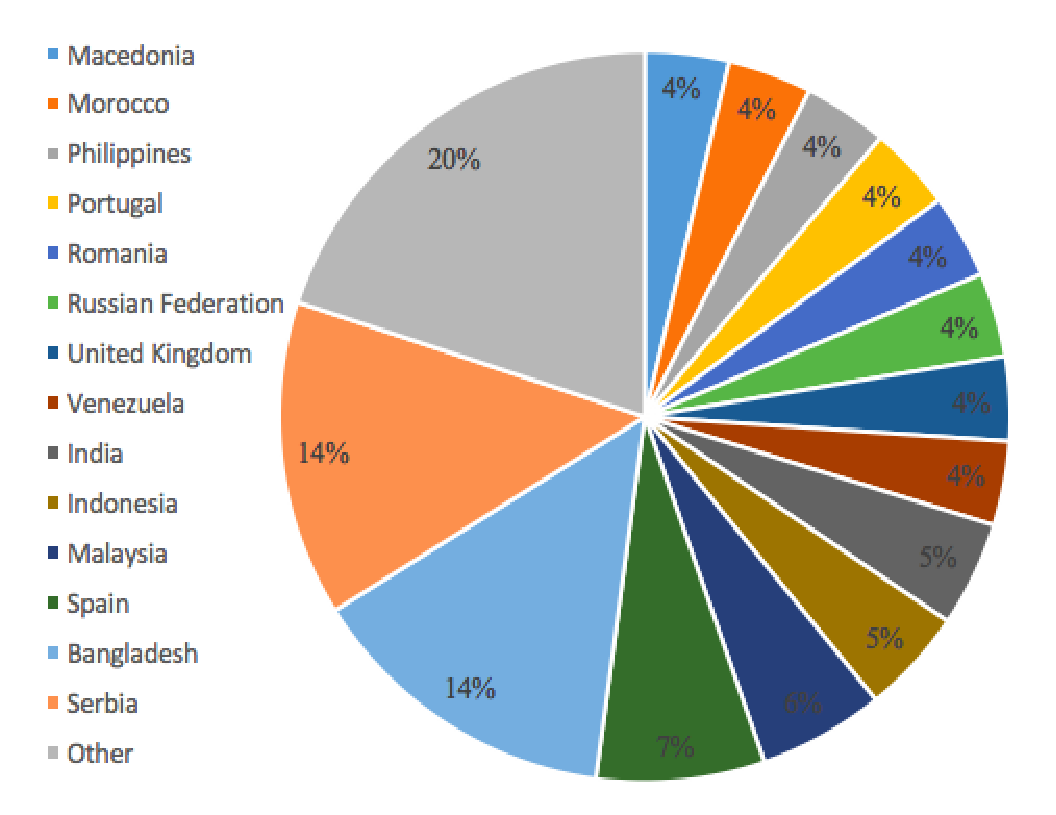
\includegraphics[scale=0.4] {figure/workers_2}}
%	\caption{Workers distribution through the world.}
%	\label{workers}
%\end{figure}

The video enrichment process has been able to produce an interactive multimedia presentation from a simple raw video through a crowdsourcing approach. This leads to the conclusion that the updated method presented is appropriate to guide this type of project that aims to generate complex media annotations.

\subsection{Issues}
Some issues were detected in relation to the collection process. About 20\% of the contributions cannot be used because they did not meet the desired specifications or because they had invalid or malicious content. This showed that it is necessary to insert in the annotation tools some resources that induce workers to provide valid contributions. It also alerted us to the importance of giving workers clearer instructions on how to properly perform tasks.

In fact, it drew attention to the need to define criteria for the evaluation of instructions given to workers. Also it brings the discussion about the need for a research on whether textual instructions are really sufficient to perform any simple annotation microtasking.

\subsection{Crowds Comparison Experiment}
Another relevant discussion from the observations of the results concerns the extent to which the composition of the crowd can influence the outcome.

To better understand, the experiment conducted will be replicated in different scenarios:
\begin{itemize}
\item Increasing the salary of workers;
\item Choosing different contracted groups;
\item Choosing only the best workers;
\item Using a closed group with volunteers;
\item Using a group familiar with the subject treated in the video;
%\item Using a group of natives in the English language.
\end{itemize}

\pagebreak

\subsection{Next Steps}

This work is constantly improving on three different fronts: improvement of the method, improvement of the system, use of the method in different scenarios and applications.

Regarding the method, the next steps include the formalization of the aggregation process, defining specific flows for automatic, supervised and manual models.

New annotation tools are being designed for the structure, which can be adapted for more tasks. In addition, a wizard is being designed to guide the creation of complex media annotation projects based on the method presented.

Some experiments are being prepared to be carried out, some of which seem especially promising:
\begin{itemize}
\item Multisensorial video annotation for mulsemedia applications.
\item Gesture segmentation in signal language video datasets.
\item Semantic approximation of idiomatic expressions in automatic translations.
\item Crowdsourcing  creation of learning object.
\end{itemize}


\begin{acks}
	The authors would like to thank the "Funda\c c\~ ao de Amparo \`a Pesquisa e Inova\c c\~ ao do Esp\'irito Santo" (FAPES) and "Coordena\c c\~ ao de Aperfei\c coamento de Pessoal de N\'ivel Superior" (CAPES).
\end{acks}



\bibliographystyle{ACM-Reference-Format}
\bibliography{refs} 

\end{document}
